\documentclass{standalone}
\usepackage{tikz}
\usetikzlibrary{patterns, positioning}
\usepackage[sfdefault]{ClearSans} %% option 'sfdefault' activates Clear Sans as the default text font
\usepackage[T1]{fontenc}

\begin{document}
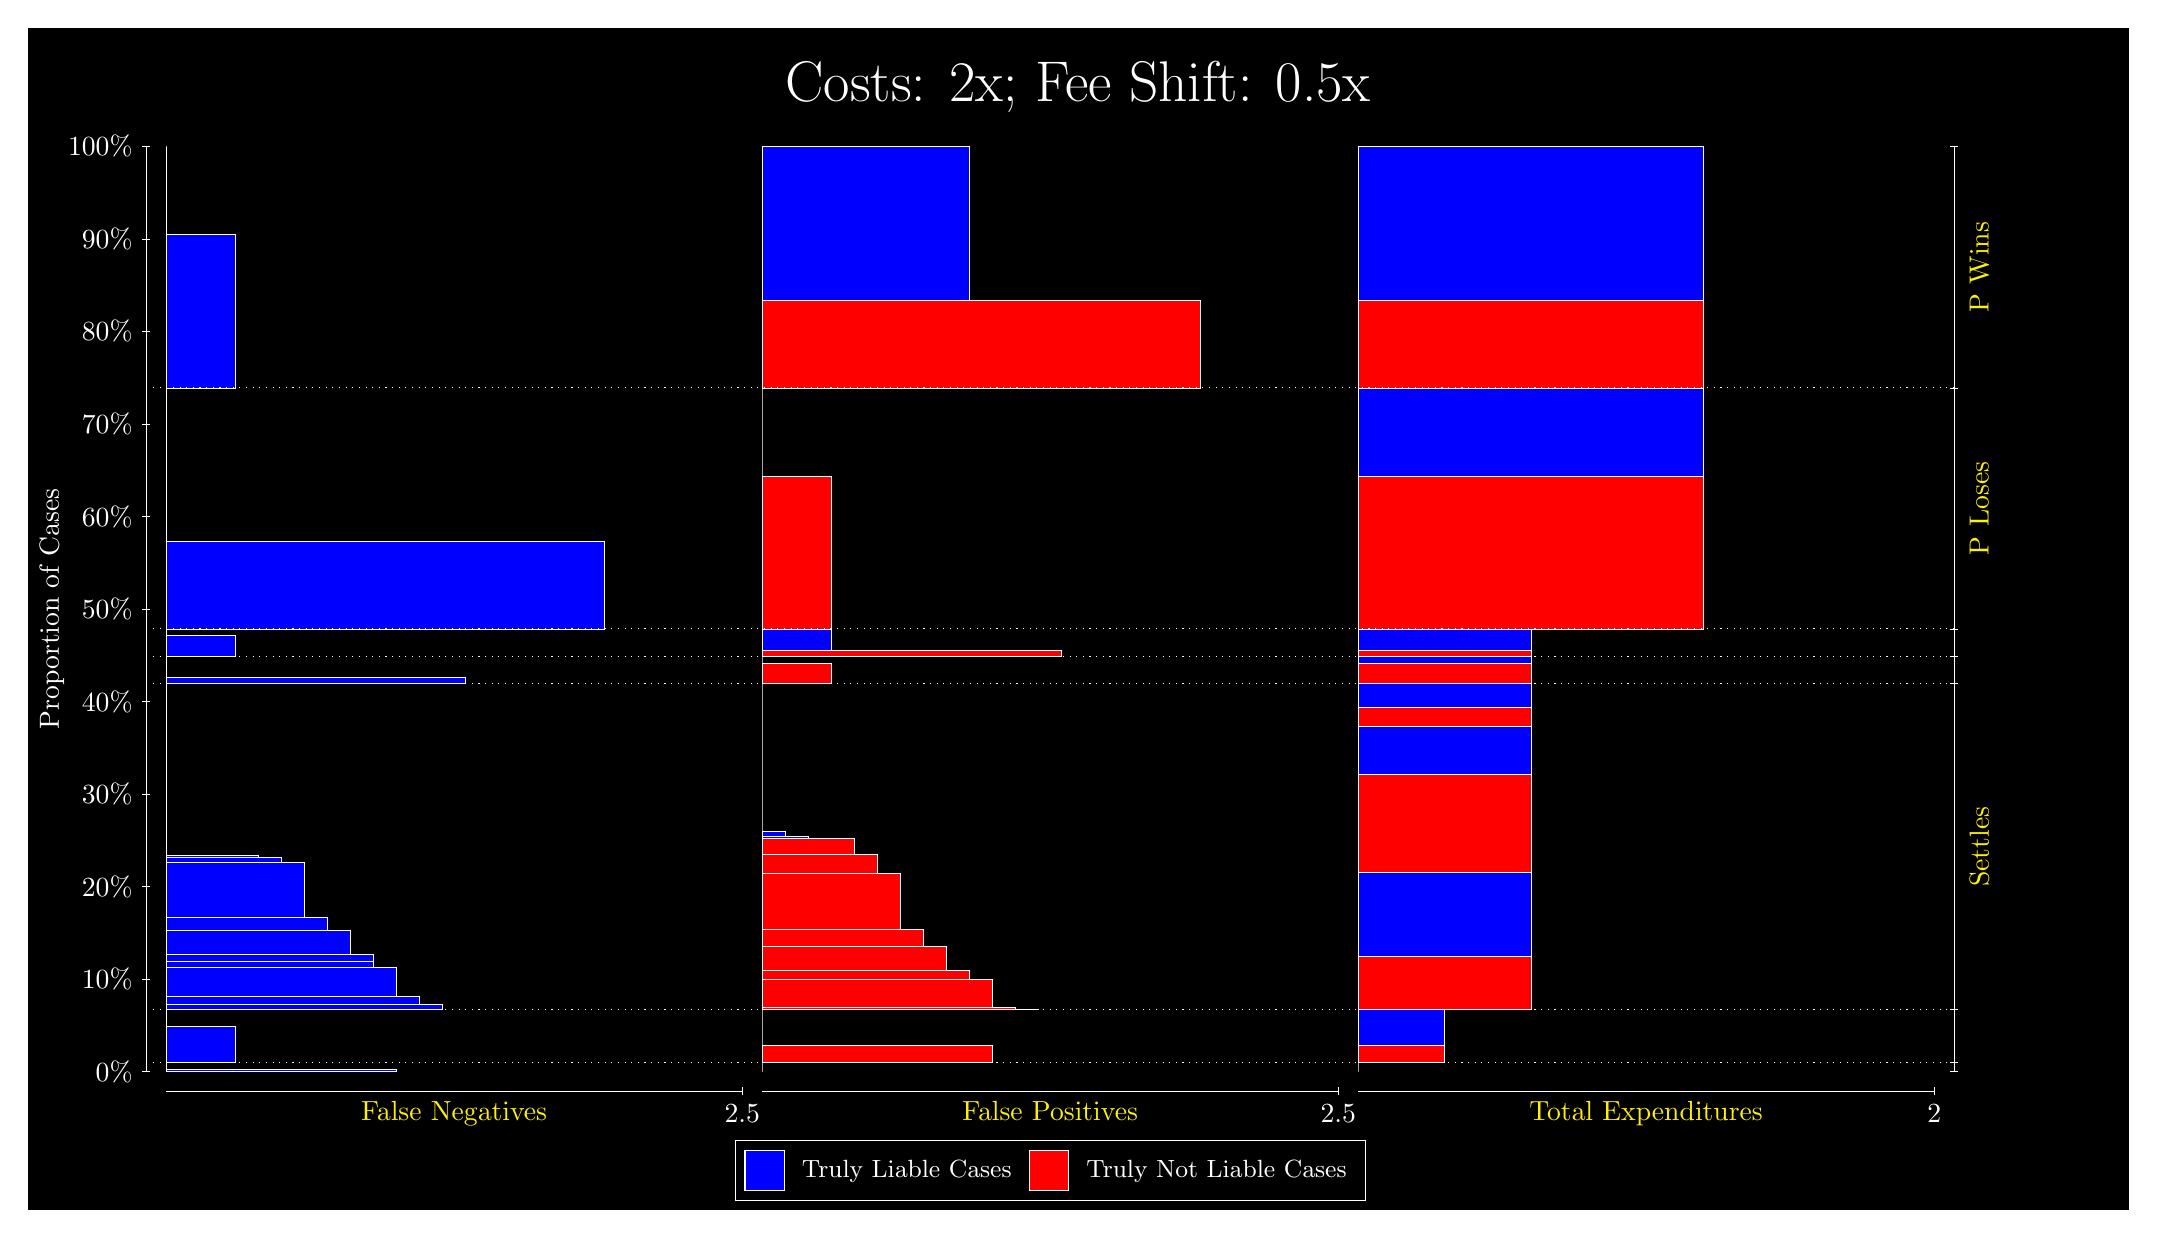
\begin{tikzpicture}
\draw[fill=black] (0,0) rectangle (26.667,15);
\draw[text=white] (0,13.5) rectangle (26.667,15) node[midway] {\huge Costs: 2x; Fee Shift: 0.5x};
\draw[white, very thin] (1.5,1.75) -- (1.5,13.5);
\node[rotate=90, text=white, anchor=center] at (0.3, 7.625) {Proportion of Cases};
\draw[white, very thin] (1.45,1.75) -- (1.55,1.75);
\node[text=white, anchor=east] at (1.45, 1.75) {0\%};
\draw[white, very thin] (1.45,2.925) -- (1.55,2.925);
\node[text=white, anchor=east] at (1.45, 2.925) {10\%};
\draw[white, very thin] (1.45,4.1) -- (1.55,4.1);
\node[text=white, anchor=east] at (1.45, 4.1) {20\%};
\draw[white, very thin] (1.45,5.275) -- (1.55,5.275);
\node[text=white, anchor=east] at (1.45, 5.275) {30\%};
\draw[white, very thin] (1.45,6.45) -- (1.55,6.45);
\node[text=white, anchor=east] at (1.45, 6.45) {40\%};
\draw[white, very thin] (1.45,7.625) -- (1.55,7.625);
\node[text=white, anchor=east] at (1.45, 7.625) {50\%};
\draw[white, very thin] (1.45,8.8) -- (1.55,8.8);
\node[text=white, anchor=east] at (1.45, 8.8) {60\%};
\draw[white, very thin] (1.45,9.975) -- (1.55,9.975);
\node[text=white, anchor=east] at (1.45, 9.975) {70\%};
\draw[white, very thin] (1.45,11.15) -- (1.55,11.15);
\node[text=white, anchor=east] at (1.45, 11.15) {80\%};
\draw[white, very thin] (1.45,12.325) -- (1.55,12.325);
\node[text=white, anchor=east] at (1.45, 12.325) {90\%};
\draw[white, very thin] (1.45,13.5) -- (1.55,13.5);
\node[text=white, anchor=east] at (1.45, 13.5) {100\%};

\draw[white, very thin] (24.457,1.75) -- (24.457,13.5);
\draw[white, very thin] (24.407,1.75) -- (24.507,1.75);
\node[anchor=west] at (24.407, 1.75) {};
\draw[white, very thin] (24.407,1.8657) -- (24.507,1.8657);
\node[anchor=west] at (24.407, 1.8657) {};
\draw[white, very thin] (24.407,2.5356) -- (24.507,2.5356);
\node[anchor=west] at (24.407, 2.5356) {};
\draw[white, very thin] (24.407,6.6759) -- (24.507,6.6759);
\node[anchor=west] at (24.407, 6.6759) {};
\draw[white, very thin] (24.407,7.0189) -- (24.507,7.0189);
\node[anchor=west] at (24.407, 7.0189) {};
\draw[white, very thin] (24.407,7.3715) -- (24.507,7.3715);
\node[anchor=west] at (24.407, 7.3715) {};
\draw[white, very thin] (24.407,10.433) -- (24.507,10.433);
\node[anchor=west] at (24.407, 10.433) {};
\draw[white, very thin] (24.407,13.5) -- (24.507,13.5);
\node[anchor=west] at (24.407, 13.5) {};

\draw[white, very thin, fill=blue] (1.75,1.75) rectangle (4.6775,1.7818);
\draw[white, very thin, fill=red] (1.75,1.7818) rectangle (1.75,1.8657);
\draw[white, very thin, fill=blue] (1.75,1.8657) rectangle (2.6283,2.3235);
\draw[white, very thin, fill=red] (1.75,2.3235) rectangle (1.75,2.5356);
\draw[white, very thin, fill=blue] (1.75,2.5356) rectangle (5.2631,2.6089);
\draw[white, very thin, fill=blue] (1.75,2.6089) rectangle (4.9703,2.7109);
\draw[white, very thin, fill=blue] (1.75,2.7109) rectangle (4.6775,3.0737);
\draw[white, very thin, fill=blue] (1.75,3.0737) rectangle (4.3848,3.144);
\draw[white, very thin, fill=blue] (1.75,3.144) rectangle (4.3848,3.2366);
\draw[white, very thin, fill=blue] (1.75,3.2366) rectangle (4.092,3.5404);
\draw[white, very thin, fill=blue] (1.75,3.5404) rectangle (3.7993,3.7138);
\draw[white, very thin, fill=blue] (1.75,3.7138) rectangle (3.5065,4.4104);
\draw[white, very thin, fill=blue] (1.75,4.4104) rectangle (3.2138,4.4702);
\draw[white, very thin, fill=blue] (1.75,4.4702) rectangle (2.921,4.5001);
\draw[white, very thin, fill=red] (1.75,4.5001) rectangle (1.75,6.6759);
\draw[white, very thin, fill=blue] (1.75,6.6759) rectangle (5.5558,6.7586);
\draw[white, very thin, fill=red] (1.75,6.7586) rectangle (1.75,7.0189);
\draw[white, very thin, fill=blue] (1.75,7.0189) rectangle (2.6283,7.288);
\draw[white, very thin, fill=red] (1.75,7.288) rectangle (1.75,7.3715);
\draw[white, very thin, fill=blue] (1.75,7.3715) rectangle (7.3123,8.4892);
\draw[white, very thin, fill=red] (1.75,8.4892) rectangle (1.75,10.433);
\draw[white, very thin, fill=blue] (1.75,10.433) rectangle (2.6283,12.385);
\draw[white, very thin, fill=red] (1.75,12.385) rectangle (1.75,13.5);
\draw[white, very thin, fill=red] (9.3189,1.75) rectangle (9.3189,1.834);
\draw[white, very thin, fill=blue] (9.3189,1.834) rectangle (9.3189,1.8657);
\draw[white, very thin, fill=red] (9.3189,1.8657) rectangle (12.246,2.0779);
\draw[white, very thin, fill=blue] (9.3189,2.0779) rectangle (9.3189,2.5356);
\draw[white, very thin, fill=red] (9.3189,2.5356) rectangle (12.832,2.5432);
\draw[white, very thin, fill=red] (9.3189,2.5432) rectangle (12.539,2.5625);
\draw[white, very thin, fill=red] (9.3189,2.5625) rectangle (12.246,2.9243);
\draw[white, very thin, fill=red] (9.3189,2.9243) rectangle (11.954,3.0338);
\draw[white, very thin, fill=red] (9.3189,3.0338) rectangle (11.661,3.3358);
\draw[white, very thin, fill=red] (9.3189,3.3358) rectangle (11.368,3.5599);
\draw[white, very thin, fill=red] (9.3189,3.5599) rectangle (11.075,4.2661);
\draw[white, very thin, fill=red] (9.3189,4.2661) rectangle (10.783,4.5132);
\draw[white, very thin, fill=red] (9.3189,4.5132) rectangle (10.49,4.7115);
\draw[white, very thin, fill=blue] (9.3189,4.7115) rectangle (9.9044,4.7413);
\draw[white, very thin, fill=blue] (9.3189,4.7413) rectangle (9.6116,4.8012);
\draw[white, very thin, fill=blue] (9.3189,4.8012) rectangle (9.3189,6.6759);
\draw[white, very thin, fill=red] (9.3189,6.6759) rectangle (10.197,6.9362);
\draw[white, very thin, fill=blue] (9.3189,6.9362) rectangle (9.3189,7.0189);
\draw[white, very thin, fill=red] (9.3189,7.0189) rectangle (13.125,7.1024);
\draw[white, very thin, fill=blue] (9.3189,7.1024) rectangle (10.197,7.3715);
\draw[white, very thin, fill=red] (9.3189,7.3715) rectangle (10.197,9.3156);
\draw[white, very thin, fill=blue] (9.3189,9.3156) rectangle (9.3189,10.433);
\draw[white, very thin, fill=red] (9.3189,10.433) rectangle (14.881,11.548);
\draw[white, very thin, fill=blue] (9.3189,11.548) rectangle (11.954,13.5);
\draw[white, very thin, fill=red] (16.888,1.75) rectangle (16.888,1.834);
\draw[white, very thin, fill=blue] (16.888,1.834) rectangle (16.888,1.8657);
\draw[white, very thin, fill=red] (16.888,1.8657) rectangle (17.986,2.0779);
\draw[white, very thin, fill=blue] (16.888,2.0779) rectangle (17.986,2.5356);
\draw[white, very thin, fill=red] (16.888,2.5356) rectangle (19.083,3.2187);
\draw[white, very thin, fill=blue] (16.888,3.2187) rectangle (19.083,4.279);
\draw[white, very thin, fill=red] (16.888,4.279) rectangle (19.083,5.5209);
\draw[white, very thin, fill=blue] (16.888,5.5209) rectangle (19.083,6.1292);
\draw[white, very thin, fill=red] (16.888,6.1292) rectangle (19.083,6.3801);
\draw[white, very thin, fill=blue] (16.888,6.3801) rectangle (19.083,6.6759);
\draw[white, very thin, fill=red] (16.888,6.6759) rectangle (19.083,6.9362);
\draw[white, very thin, fill=blue] (16.888,6.9362) rectangle (19.083,7.0189);
\draw[white, very thin, fill=red] (16.888,7.0189) rectangle (19.083,7.1024);
\draw[white, very thin, fill=blue] (16.888,7.1024) rectangle (19.083,7.3715);
\draw[white, very thin, fill=red] (16.888,7.3715) rectangle (21.279,9.3156);
\draw[white, very thin, fill=blue] (16.888,9.3156) rectangle (21.279,10.433);
\draw[white, very thin, fill=red] (16.888,10.433) rectangle (21.279,11.548);
\draw[white, very thin, fill=blue] (16.888,11.548) rectangle (21.279,13.5);
\draw[white, dotted] (1.5,1.8657) -- (24.457,1.8657);
\draw[white, dotted] (1.5,2.5356) -- (24.457,2.5356);
\draw[white, dotted] (1.5,6.6759) -- (24.457,6.6759);
\draw[white, dotted] (1.5,7.0189) -- (24.457,7.0189);
\draw[white, dotted] (1.5,7.3715) -- (24.457,7.3715);
\draw[white, dotted] (1.5,10.433) -- (24.457,10.433);
\draw[white, very thin] (1.75,1.5) -- (9.0689,1.5);
\node[text=yellow, anchor=north] at (5.4094, 1.5) {False Negatives};
\draw[white, very thin] (9.0689,1.45) -- (9.0689,1.55);
\node[text=white, anchor=north] at (9.0689, 1.45) {2.5};

\draw[white, very thin] (9.3189,1.5) -- (16.638,1.5);
\node[text=yellow, anchor=north] at (12.978, 1.5) {False Positives};
\draw[white, very thin] (16.638,1.45) -- (16.638,1.55);
\node[text=white, anchor=north] at (16.638, 1.45) {2.5};

\draw[white, very thin] (16.888,1.5) -- (24.207,1.5);
\node[text=yellow, anchor=north] at (20.547, 1.5) {Total Expenditures};
\draw[white, very thin] (24.207,1.45) -- (24.207,1.55);
\node[text=white, anchor=north] at (24.207, 1.45) {2};



\node[text=yellow, centered, rotate=90] at (24.777, 4.6058) {Settles};


\node[text=yellow, centered, rotate=90] at (24.777, 8.9024) {P Loses};
\node[text=yellow, centered, rotate=90] at (24.777, 11.967) {P Wins};

\draw (12.978300999999998,1.5) node[draw=none] (baseCoordinate) {};
\begin{scope}[align=center]
        \matrix[scale=0.5, draw=white, below=0.5cm of baseCoordinate, nodes={draw}, column sep=0.1cm]{
            \node[rectangle, draw, minimum width=0.5cm, minimum height=0.5cm, fill=blue] {}; &
            \node[draw=none, font=\small, text=white] (B) {Truly Liable Cases}; &
            \node[rectangle, draw, minimum width=0.5cm, minimum height=0.5cm, fill=red] {}; &
            \node[draw=none, font=\small, text=white] (B) {Truly Not Liable Cases}; \\
            };
\end{scope}

\end{tikzpicture}
\end{document}